\documentclass{article}
\usepackage{hyperref}
\usepackage{tikz}
\usepackage{python}
\usepackage[%
    natbib=true,%
    backend=biber,%
    backref=true,%
    citestyle=authoryear-comp,%
    bibstyle=authoryear,%
    maxbibnames=24,%
    maxcitenames=2,%
]{biblatex}

\hypersetup{%
    bookmarks=true,
    colorlinks=true,
    pdfauthor={Luis Pedro Coelho},
    citecolor=pondgreen,
    urlcolor=toastedchilipowder,
    linkcolor=toastedchilipowder,
}
\newcommand*{\cpp}{{C\nolinebreak[4]\hspace{-.05em}\raisebox{.4ex}{\tiny\textbf{++}}}}
\let\code\texttt
\addbibresource{references.bib}

\title{Mahotas: Open source software for scriptable computer vision}
\author{Luis Pedro Coelho\\
Lane Center for Computational Biology, Carnegie Mellon University, Pittsburgh, USA\\
Instituto de Medicina Molecular, Lisboa, Portugal}

\begin{document}
\maketitle

\section*{Abstract}
Mahotas is a computer vision library for Python. It contains traditional image
processing functionality such as filtering and morphological operations as well
as more modern computer vision functions for feature computation, including
local features.

The interface is in Python, a dynamic programming language, which is very
appropriate for fast development, but the algorithms are implemented in \cpp{}
and are tuned for speed.

Mahotas is available under a liberal open source license (MIT License) and is
available from \url{http://github.com/luispedro/mahotas} or the Python Package
Index (\url{http://pypi.python.org/pypi/mahotas}).

\textbf{Keywords:} computer vision, image processing.

\section{Introduction}

Mahotas is a computer vision library for the Python Programming Language
(versions 2.5 and up, including version 3). It operates on numpy
arrays~\citep{numpystructure}. Therefore, it uses all the infrastructure built
by that project for storing information. In particular, unlike libraries
written in the C~Language or in Java~\citep{Marcel:2010:TMP:1873951.1874254},
Mahotas does not need to define a data structure, but uses the numpy array
structure. Many basic manipulation functionality that would otherwise be part
of a computer vision library are handled by numpy, for example computing
averages and other simple statistics, handling multi-channel images, converting
between types (integer and floating point images are supported by mahotas,
whenever it is meaningful). For the user, this has the additional advantage
that they do not need to learn yet another set of functions.

On the other end, by integrating into the Python numeric ecosystem, users can
use other packages in a seamless way. In particular, mahotas does not implement
any machine learning functionality, but rather advises the user to use another,
specialised package, such as scikits-learn or milk.

Python is a natural ``glue'' language: it is easy to use state-of-the-art
libraries written in multiple languages~\citep{10.1109/MCSE.2007.58}. Mahotas
itself is a mix of high-level Python and low-level \cpp{}. This achieves a good
balance between speed and ease of implementation.

Version 1.0 of mahotas has been released recently and this is now a mature,
well-tested package (the first version was made available over 4~years ago).
\footnote{Note for reviewers: the version currently available implements all
functionality described in this manuscript. I will release it as version 1.0
when this manuscript is accepted to coincide with publication. Naturally, any
bugs that are found and reported in the meanwhile will be addressed.} Mahotas
runs and is used on different versions of Unix (including Linux, SunOS, and
FreeBSD), Mac OS X, and Windows.

\section{Implementation and Architecture}

\subsection{Interface}

The interface is a procedural interface, with no global state. All functions
work independently of each other (there is code sharing at the implementation
level, but this is hidden from the user).

The main functionality is grouped into the following categories:

\begin{description}
\item[\textsc{surf}] Speeded-up Robust Features~\citep{eth_biwi_00517}. This
includes both keypoint detection and descriptor computation.
\item[features] Global feature descriptors. In particular, Haralick texture
features, Zernike moments, local binary patterns, and threshold adjacency
statistics (both the original~\citep{Hamilton2007} and the parameter-free
versions~\citep{Coelho2010}).
\item[Wavelet] Haar and Daubechies wavelets. Forward and inverse transforms.
\item[morphological functions] Erosion and dilation, as well as some more
complex operations built on these. There are both binary and grayscale
implementations of these operators.
\item[watershed] seeded watershed and distance map
transforms~\citep{felzenszwalb}.
\item[filtering] Gaussian filtering and general convolutions.
\item[polygon operations] convex hull, polygon drawing.
\end{description}

In general, functions operate on all data types (in some cases, the operation
is only meaningful for floating point arrays, for example). This is performed
without any extra memory copies. Mahotas is heavily optimised for both speed
and memory usage (it can be used with very large arrays).

There are a few interface conventions which apply to many functions. When
meaningful, a structuring element is used to define neighbourhoods or adjacency
relationships (morphological functions, in particular, use this convention).
Generally, the default is to use a $3 \times 3$ cross as the default if no
structuring filter is given (the exception to this rule is the median filter,
where the default is a $3 \times 3$ square).

When a new image is to be returned, functions take an argument named \code{out}
where the output will be stored. This argument is often much more restricted in
type. In particular, it must often be a contiguous array.\footnote{Numpy
supports non-contiguous arrays, which are most often slices into other, larger,
contiguous arrays (e.g., given a $128 \times 128$ contiguous array, one can
build a $64 \times 128$ non-contiguous array by taking every other row).} Since
this is a performance feature (its purpose is to avoid extra memory
allocation), it is natural that the interface is less flexible (accessing a
contiguous array is much more efficient than a non-contiguous one).

\subsection{Example of Use}

This is a simple example of mahotas usage. Code for this and other examples is
present in the mahotas source distribution under the \texttt{demos/} directory.
In this example, we load an image and find SURF interest point and descriptors
on it.

We start by importing the necessary packages, including numpy and mahotas. We
also use \textit{milk}, to demonstrate how the mahotas output can integrate
with a machine learning package.

\begin{python}
import numpy as np
import mahotas
from mahotas.features import surf
import milk
\end{python}

The first step is to load the image and convert to 8~bit numbers. In this
case, the conversion is done using standard numpy methods, namely
\code{astype}:

\begin{python}
f = mahotas.imread('luispedro.jpg', as_grey=True)
f = f.astype(np.uint8)
\end{python}

We can now compute SURF interest points and descriptors.
\begin{python}
spoints = surf.surf(f, 4, 6, 2)
\end{python}

Using numpy operations and milk, we can select only the descriptors and cluster
them into a group of five:

\begin{python}
descrs = spoints[:,6:]
values, _ = milk.kmeans(descrs, 5)
\end{python}

Finally, we can show the points in colour.
\begin{python}
colors = np.array(
    [ 255,  25,   1],
    [203,  77,  37],
    [151, 129,  56],
    [ 99, 181,  52],
    [ 47, 233,   5]])
f2 = surf.show_surf(f, spoints[:64], values, colors)
\end{python}

The \texttt{show\_surf} only builds the image as a multi-channel (one for each
colour) image. Using matplotlib~\citep{10.1109/MCSE.2007.55}, we finally
display the image as Figure~\ref{fig:surf}.

\begin{python}
from matplotlib import pyplot as plt
plt.subplot(1,2,1)
plt.imshow(f)
plt.subplot(1,2,2)
plt.imshow(f2)
\end{python}

The easy interaction with matplotlib is another way in which we benefit from
the numpy-based ecosystem.

\begin{figure}
\begin{center}
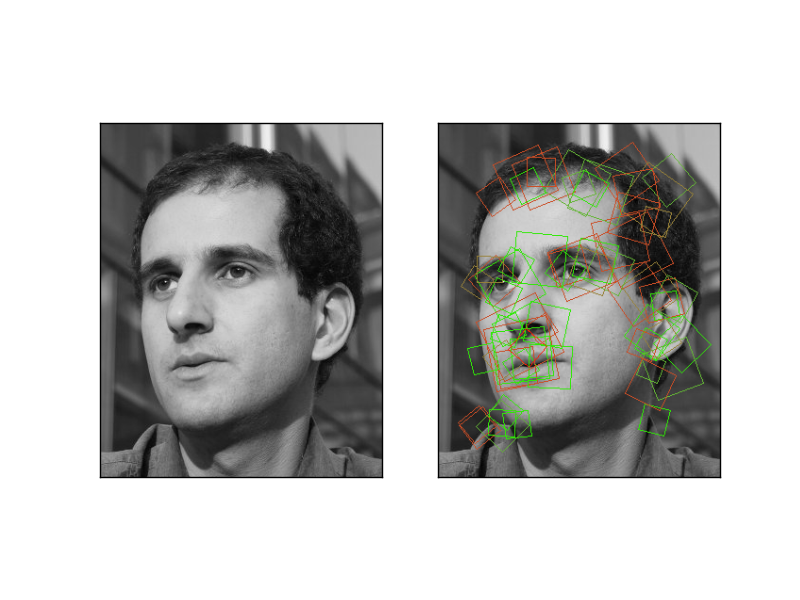
\includegraphics[width=.8\textwidth]{surf-tutorial}
\end{center}
\caption{Example of Usage. On the left, the original image is shown, while on
the right SURF detections are represented as rectangles of different colours.}
\label{fig:surf}
\end{figure}

\subsection{Implementation}

Mahotas is mostly written in \cpp, but this is completely hidden from the user
as there are hand-written Python wrappers for all functions (automatically
generated wrappers inevitably lead to worse error messages and are less
flexible).

The main reason that mahotas is implemented in \cpp{} (and not in C, which is
the language of the Python interpreter) is to use templates. Almost \cpp{}
functionality is split across 2~functions:

\begin{enumerate}
\item A \code{py\_function} which uses the Python C~API to get arguments and
check them.
\item A template \code{function<dtype>} which works for the type \code{dtype}
performing the actual operation.
\end{enumerate}

So, for example, this is how \emph{erode} is implemented. \code{py\_erode}
consists mostly of boiler-plate code:

\begin{cplusplus}
PyObject* py_erode(PyObject* self, PyObject* args) {
    PyArrayObject* array;
    PyArrayObject* Bc;
    if (!PyArg_ParseTuple(args,"OO", &array, &Bc)) {
        return NULL;
    }
    PyArrayObject* res_a = (PyArrayObject*)PyArray_SimpleNew(
                                array->nd,
                                array->dimensions,
                                PyArray_TYPE(array));
    if (!res_a) return NULL;
    PyArray_FILLWBYTE(res_a, 0);
    switch(PyArray_TYPE(array)) {
#define HANDLE(type) \
    erode<type>(numpy::aligned_array<type>(res_a), \
                numpy::aligned_array<type>(array), \
                numpy::aligned_array<type>(Bc));

        HANDLE_INTEGER_TYPES();
#undef HANDLE
    ...
\end{cplusplus}

This functions retrieves the arguments, performs some sanity checks, performs a
bit of initialisation, and finally, switches in the input type with the help of
the \code{HANDLE\_INTEGER\_TYPES()} macro, which call the right specialisation
of the template that does the actual work. In this example \code{erode}
implements (binary) erosion:

\begin{cplusplus}
template<typename T>
void erode(numpy::aligned_array<T> res,
            numpy::aligned_array<T> array,
            numpy::aligned_array<T> Bc) {
    gil_release nogil;
    const unsigned N = res.size();
    typename numpy::aligned_array<T>::iterator iter = array.begin();
    filter_iterator<T> filter(res.raw_array(), Bc.raw_array());
    const unsigned N2 = filter.size();
    T* rpos = res.data();

    for (int i = 0;
                i != N;
                ++i, ++rpos, filter.iterate_both(iter)) {
        for (int j = 0; j != N2; ++j) {
            T arr_val = false;
            filter.retrieve(iter, j, arr_val);
            if (filter[j] && !arr_val) {
                goto skip_this_one;
            }
        }
        *rpos = true;
        skip_this_one: continue;
    }
}
\end{cplusplus}

The template machinery makes the functions that use it very simple and easy to
read. The only downside is that there is some expansion of code size when the
compiler instanciates the function for the several integer and floating point
types. Given the small size of these functions, this is not a big issue.

In the snippet above, you can see some other \cpp{} machinery:

\begin{description}
\item[\code{gil\_release}] This is a ``resource-acquisition is object
initialisation'' (\textsc{raii})\footnote{\textsc{Raii} is a design pattern in
\cpp{}, or other languages with scope linked deterministic object destruction,
such as D, where a resource is represented by an object, whose constructor
acquires it and whose destructor releases it. This guarantees that the object
is correctly released even if the scope is left through an exception
\citep{Stroustrup1994}.} object that release the Python global interpreter lock
(\textsc{gil})\footnote{In the CPython interpreter, the most commonly used
implementation of Python, there is a global lock for many Python related
functionality, which limits parallelism.} in its constructor and gets it back
in its destructor. Normally, the template function will release the
\textsc{gil} after the Python-specific code is done. This allows several
mahotas functions to run concurrently.
\item[\code{array}] This is a thin wrapper around \code{PyArrayObject} that
knows its data type and has iterators which resemble the \cpp{} standard
library. This makes the code type-safer. This is also a \textsc{raii} object in
terms of managing Python reference counts.
\item[\code{filter\_iterator}] This is taken from \code{scipy.ndimage} and it
is useful to iterate over an image and use a centered filter around each pixel
(it keeps track of all of the boundary conditions).
\end{description}

The inner loop is as direct an implementation of erosion as one would wish for:
for each pixel in the image, look at its neighbours. If all are true, then set
the corresponding output pixel to \textbf{true} (else, skip it as it has been
initialised to zero).

In keeping with the philosophy of blending in with the ecosystem, Mahotas uses
the standard Python build machinery and distribution channels. Building and
installing from source code is done using
\begin{verbatim}
python setup.py install
\end{verbatim}
Alternatively, Python based package managers (such as \texttt{easy\_install} or
\texttt{pip}) can be used (mahotas works well with these systems).

\subsection{Quality Control}

Mahotas includes a complete automated suite of unit tests. These all
functionality and include several regression tests. There are no known bugs in
version~1.0. In fact, no releases have ever been performed with known bugs.
Naturally, bugs were, occasionally, discovered in released versions, but
corrected before the next release.

The development is completely open-source and development versions are
available. Many users have submitted bug reports and fixes.

\section{Availability}

\textbf{Operating system}\\
Mahotas runs and is used on different versions of Unix (including Linux, SunOS,
and FreeBSD), Mac OS X, and Windows.


\textbf{Programming language}\\
Mahotas works in Python (minimal version is~2.5 and works in all more recent
versions, including in the Python~3 series).

\textbf{Additional system requirements}\\
None.

\textbf{Dependencies}\\
It requires numpy to be present and installed.


\textbf{List of contributors}\\
Luis Pedro Coelho (Carnegie Mellon University and Instituto de Medicina
Molecular), Zachary Pincus (Stanford University), Peter J. Verveer (European
Molecular Biology Laboratory), Davis King (Northrop Grumman ES), Robert Webb
(Carnegie Mellon University), Matthew Goodman (University of Texas at Austin),
K.-Michael Aye (University of Bern), Rita Sim\~{o}es (University of Twente),
Joe Kington (University of Wisconsin), Christoph Gohlke (University of
California, Irvine), and Sandro Knauss (University of Bremen).

\subsubsection{Software location}

\textbf{Code repository}\\
\textit{Name}: Github\\
\textit{Identifier}: https://github.com/luispedro/mahotas\\
\textit{Licence}: MIT\\
\textit{Date published}: Since 2009

\section{Discussion}

Mahotas does not include machine learning related functionality, such as
$k$-means clustering or any classification. This is the result of an explicit
design decision. Specialised machine learning packages for Python already
exist~\citep{Pedregosa:2011:SML:2078183.2078195,springerlink:10.1007/978-3-540-30116-5_58,Schaul:2010:PYB:1756006.1756030,Sonnenburg:2010:SML:1756006.1859911}.
A good classification (or other) system can benefit both computer vision users
and others. As these projects all use Numpy arrays as their data types, it is
easy to use functionality from the different project seamlessly (no copying of
data is necessary).

Python is an ideal language for fast development of both applications and
scientific software. For this platform, Mahotas is a fast library of computer
vision and image processing functions. It is implemented in \cpp{}, as the
standard Python interpreter is too slow for a direct Python implementation.
However, all of the Python interface code is hand-written, as opposed to using
automatic interface generators like Swig~\cite{Beazley2003599}. This is more
work, but the end result is of much higher quality, especially when it comes to
giving useful error messages (e.g., when a type mismatch occurs, an automatic
system will often be forced to resort to a generic message as it does not have
any knowledge of what the arguments mean besides their automatically inferred
types).

Mahotas has been available in the Python Package Index since April~2010 and has
been downloaded over 20,000~times. This does not include any downloads from
other sources. Mahotas includes a full test suite (version 1.0 has 100\% test
coverage). There are no known bugs.

\section{Reuse Potential}

Originally, this code was developed in the context of cellular image analysis.
However, none of the functionality is specific to this context and many
computer vision pipelines can make use of it.

This package (and earlier versions of it) have been used by
myself~\citep{Coelho2009,Coelho2010a} and close collaborators in several
publications~\citep{omerosearcher}. Other groups have used in published work,
both in cell image analysis~\citep{CYTO:CYTO22034} and in other
areas~\citep{springerlink:10.1007/978-3-642-32335-5_2}.

\subsection*{Acknowledgements}

Mahotas includes code ported and incorporated from other projects. In
particular, the \textsc{surf} implementation is a port from the code from
\textit{dlib},\footnote{Dlib's webpage is at \url{http://dlib.net}.} a very
good \cpp{} library by Davis King. I also gleaned some insight into the
implementation of these features from Christopher Evan's OpenSURF library and
its documentation \citep{evans2009}.\footnote{OpenSURF is available at
\url{http://www.chrisevansdev.com/computer-vision-opensurf.html}, where several
documents describe details of the implementation.} The code which interfaces
with the FreeImage library, was written by Zachary Pincus and some of the
support code was written by Peter J. Verveer for the \code{scipy.ndimage}
project. All of these contributions were integrated while respecting the
software licenses under which the original code had been released. Robert Webb,
a summer student at Carnegie Mellon University, worked with me on the initial
local binary patterns implementation. Finally, I thank the several users who
have reported bugs, submitted small fixes, and participated on the project
mailing list.

\textbf{Funding}: I was supported in my work by the Funda\c c\~{a}o para a
Ci\^encia e Tecnologia (grants SFRH/BD/37535/2007 and PTDC/SAU-GMG/115652/2008)
and by a grant from the Siebel Scholars Foundation.


\printbibliography
\end{document}
